%% Change "letterpaper" in the following line to "a4paper" if you must.

\documentclass[10pt,a4paper]{article}
\usepackage{cogsci}
\usepackage{pslatex}
\usepackage{apacite}


%\usepackage{geometry}
\usepackage{natbib}
\bibpunct[:]{(}{)}{,}{a}{}{;}

\usepackage{amsmath}
\usepackage{amsfonts}
\usepackage{amsthm}
\usepackage{amssymb}
\usepackage{mathrsfs}
\usepackage{nicefrac}
%\usepackage{stmaryrd}
%\usepackage{multicol}
\usepackage{graphicx}
\usepackage{caption}
\usepackage{subcaption}
\usepackage{color}
\usepackage{booktabs}

\usepackage{blkarray}
\usepackage{xspace}


\definecolor{Red}{RGB}{178,34,34}
\newcommand{\mf}[1]{\textcolor{Red}{[MF: #1]}} 
\newcommand{\tb}[1]{\textcolor[rgb]{.8,.33,.0}{[TB: #1]}}% prints in orange
\newcommand{\citeposs}[2][]{\citeauthor{#2}'s (\citeyear[#1]{#2})}
\newcommand{\tuple}[1]{\ensuremath{\left\langle #1 \right\rangle}} 


%%% MF's commands
\newcommand{\set}[1]{\left\{#1\right\}}
\newcommand{\card}[1]{\left \lvert \, #1 \, \right\rvert}
\newcommand{\abs}[1]{\lvert #1 \rvert}
\newcommand{\States}{\ensuremath{S}\xspace}		% Set of States
\newcommand{\state}{\ensuremath{s}\xspace}		% single states
\newcommand{\mystate}[1]{\ensuremath{\state_{\text{#1}}}\xspace} %meaningful states
\newcommand{\Messgs}{\ensuremath{M}\xspace}		% Set of Messages
\newcommand{\messg}{\ensuremath{m}\xspace}		% single messages
\newcommand{\mymessg}[1]{\ensuremath{\messg_{\text{#1}}}\xspace} %meaningful messages
\newcommand{\ssome}{\mystate{\ensuremath{\exists\neg\forall}}}
\newcommand{\sall}{\mystate{\ensuremath{\forall}}}
\newcommand{\msome}{\mymessg{some}}
\newcommand{\mall}{\mymessg{all}}
\newcommand{\asome}{\myact{\ensuremath{\exists\neg\forall}}}
\newcommand{\aall}{\myact{\ensuremath{\forall}}}
\definecolor{mygray}{cmyk}{0.35,0.35,0.35,0.35}
\newcommand{\mygray}[1]{{\textcolor{mygray}{#1}}}


%\citeA{bibkeyword} cites only year

\title{Systematic transmission perturbations in the cultural evolution of language}
 
\author{{\large \bf Name Surname (mail@mail.com)} \\
  Department, street \& number \\
  city, ZIP country
  \AND {\large \bf Name Surname (mail@mail.com)} \\
  Department, street \& number \\
  city, ZIP country}


\begin{document}
\maketitle

\begin{abstract}
Over time, languages favors linguistic features that can be passed on with high fidelity from one language user to the next. The outcomes of this process are often argued to involve cognitive biases that influence a learner's inductive task. Such learning biases thereby serve as central devices to understand and predict linguistic structure. We complement this view by showing how such outcomes can also arise without assuming any biases but simply as an epiphenomenon of systematic disturbances stemming from environmental factors. To this end, we investigate the effects of iterated learning under noisy perception in three case studies on (i) vagueness, (ii) meaning deflation, and (iii) a lack of upper-bounds in weak scalar expressions. These results underpin and elucidate the importance of, either cognitive or extraneous, transmission perturbations in the cultural evolution of language and bring attention to the often overlooked possibility that channel noise can mimic effects of inductive biases.

\textbf{Keywords:} 
noise; cognitive biases; iterated learning; cultural evolution;  
\end{abstract}
\section{Introduction}
Language is shaped by its use and transmission across generations. Linguistic properties therefore need not necessarily arise and stabilize solely due to functional pressure but may also be influenced and selected for by a pressure for learnability. The effects that (iterated) learning has on language are often seen as stemming from a combination of general learning mechanisms and inductive cognitive biases (e.g. \citealt{griffiths+kalish:2007,kirby+etal:2014,tamariz+kirby:2016}). Proposals of biases that shape language acquisition abound. Some prominent examples are mutual exclusivity \citep{merriman+bowman:1989,clark:2009}, simplicity \citep{kirby+etal:2015}, regularization \citep{hudson+etal:2005}, and generalization \citep{smith:2011,oconnor:2015}.\footnote{Depending on their formulation and the domain(s) they are proposed to apply to, biases may also interact. For instance, a domain-independent bias for simplicity may entail regularization but stand in conflict with mutual exclusivity.} In the following we show how environmental factors can produce evolutionary outcomes that look as if such learning biases are present even if they are not.

We present three case studies that show how transmission perturbations can lead to the emergence of vagueness, meaning deflation, and a lack of upper-bounds in weak scalar expressions in populations of language users. These results are not meant to suggest noisy perception to be the sole or main determinant of these phenomena. Instead, this investigation's main contribution is conceptual and technical in nature in that it aims to clarify the role of systematic transmission perturbations of linguistic knowledge in language change while showing that such perturbations may stem from other sources, e.g., from learners' noisy perception.


\section{Iterated learning under noisy perception}
We model the transmission of linguistic knowledge as a process of iterated learning (for recent overviews see \citealt{kirby+etal:2014, tamariz+kirby:2016}). That is, as a repeated transfer of knowledge and behavior, such a language and its use, from one agent to another. 

In the simplest case one may think of this process as involving a chain of parents and children. At the chain's top a parent produces linguistic data. This data is witnessed by the next agent in the chain, a child, who acquires a language and behavior based on it. This agent, now turned a proficient language user, then goes on to produce data for the next child in the chain to learn from, and so on. The learner's task is therefore to infer covert linguistic information from observable language use. Importantly, there are multiple ways in which this process can induce change in a language. Among others, learning data may be sparse, speakers may make mistakes in production, or it could be that the data incorrectly perceived by the learner. The fidelity by which linguistic features are transmitted against such perturbations therefore plays an important role in their emergence and stability across generations.

If linguistic behavior is constant across agents then the learner's task reduces to that of inferring a language. A more general approach is to allow for variation in the agents' production algorithm as well \citep{brochhagen+etal:2016:CogSci}. In such cases the learner performs a joint inference over types of linguistic behavior and languages. We call such a combination a type, $t \in T$. 

More precisely, we follow \citet{griffiths+kalish:2007} in modeling language acquisition as a form of (iterated) Bayesian learning. Learning is hereby represented as a combination of the likelihood of a type generating the data witnessed by the learner with prior inductive biases, $P \in \Delta(T)$. This prior can be understood as a condensed codification of a learner's a priori preferences. For example, learners may have a preference for simpler languages over ones with a more complex grammar, larger or more marked inventories, or cognitively taxing components (c.f. \citealt{feldman:2000,chater+vitanyi:2003, kirby+etal:2015}). Crucially, even weak biases can magnify and have striking effects on an evolving linguistic system. Experimental and mathematical investigations in iterated learning have therefore argued that the linguistic structure evinced by the outcome of this process reflect learners' inductive biases \citep{kirby+etal:2007,kirby+etal:2014}. The role of such biases can be viewed as that of introducing systematic perturbations in the transmission of linguistic knowledge, guiding learners to the convergence on particular evolutionary outcomes. In the following, we show how environmental factors can play a similar role. To this end, we introduce a variant of iterated Bayesian learning that gives room for environmental perturbations in the learning process. 

Informally, the idea is that agents may not always perceive states of affairs perfectly. Such noisy perception may lead parents to produce utterances that deviate from their production behavior -- had they witnessed the state correctly. Similarly, children may mistake utterances as applying to a different state than the one witnessed by the parent who produced it. For instance, when learning the meaning of a vague adjective such as {\em tall}, agents may have trouble discerning small differences in height between objects, leading to their occasional confusion.

Let $S$ be a set of states of affairs or meanings. We denote the probability that the teacher (learner) observes state $s_t$ ($s_l$) when the actual state is $s_a$ as $P_N(s_t \mid s_a)$ ($P_N(s_l \mid s_a)$). The probability that $s_a$ is the actual state when the learner observes $s_l$ is therefore:
\begin{align*}
  P_N(s_a \mid s_l) \propto P(s_a) \ P_N(s_l \mid s_a)\,.
\end{align*}

Accordingly, the probability that the teacher observes $s_t$ when the learner observes $s_l$ is:
\begin{align*}
  P_N(s_t \mid s_l) = \sum_{s_a} P(s_a \mid s_l) \ P_N(s_t \mid s_a)\,.
\end{align*}

Noise free iterated Bayesian learning is obtained as a special case when the perceived state is always the actual state. 

The set of possible data a learner may be exposed to is represented by a set $D$. This set is made up of $k$-length sequences of the form $\tuple{\tuple{s_i,m_j}, ..., \tuple{s_k,m_l}}$, where $s \in S$ is the observation of state $s$ accompanied with an utterance $m \in M$. The parameter $k$ therefore controls how much information learners have at their disposition. Generally, low $k$ means that more types will be compatible with the data, lowering the likelihood of a particular type being passed on faithfully. Conversely, inferring the type that generated the data, i.e., adopting the teacher's type , has a higher likelihood for larger sequences. Factoring in noisy perception in production and comprehension, the probability that a teacher of type $t$ produces a datum that is
perceived by the listener as $d = \tuple{s_l, m}$ is:
\begin{align*}
  P_N(\tuple{s_l, m} \mid t) = \sum_{s_t} P_N(s_t \mid s_l) \ P(m \mid s_t; t)\,.
\end{align*}

%The likelihood $P(d|t_j)$ of datum $d$ being produced by type $t_j$ is given by a parent $j$'s linguistic behavior in combination with the language it uses. Letting $P_{PA_j}(\cdot)$ and $L_j$ stand type $j$'s production algorithm and language:
%
%\begin{align*}
%  P(d = \tuple{\tuple{s_1,m_1},\dots , \tuple{s_k,m_k}} \mid t_j) = \prod_{i = 1}^k P_{PA_j}(m_i
%  \mid s_i; L_{j})\,.
%\end{align*}
%


Generalize this to a sequence of perceived data $d_l$ and write $P_N(d_l \mid t)$. These components can then be put together in a transmission matrix $Q$, where $Q_{ji}$ is the probability that a learner acquires type $i$ when learning from type $j$
\begin{flalign*}
  Q_{ji} \propto \sum_{d \in D} P(d_l \mid t_j) F(t_i \mid d)\,,
\end{flalign*}

where $F(t_i \mid d)$ is the parametrized acquisition probability of $t_i$ given datum $d$, obtained from the likelihood and prior:
\begin{flalign*}
  & F(t_i \mid d) \propto [P(t_i) P(d \mid t_i)]^l\,,
\end{flalign*}

where $l \geq 1$ is a posterior parameter. This parameter controls how learners select types from the posterior. If $l = 1$ learners sample from it. As $l$ increases so does the learner's propensity to maximize the posterior \citep{griffiths+kalish:2007, kirby+etal:2007}. Consequently, the model accommodates an infinite number of learning strategies and a value of $l$ instantiates a particular one, with posterior sampling and maximum a posterior estimation serving as the two extremes of the learning spectrum. 


Finally, we need to specify what the transmission matrix $Q$ operates over. This could be a distribution over types that an agent in the learning chain entertains at a given time, but also as a population of types following standard practice in evolutionary game theory (for discussion on the relationship of single chain learning and population dynamics see e.g. \citealt[\S 7]{griffiths+kalish:2007}). Here, we adopt the latter view, and consequently take this component to be a population vector $x$, where $x_i$ is the proportion of type $t_i$ in $x$. The full dynamics are captured by the discrete mutator dynamics $\hat{x}_j = \sum_i Q_{ij} x_j$ (for an overview see \citealt{hofbauer+sigmund:2003}).

In sum, it may be the case that learner and/or teacher do not perceive the actual state as what it is. They are not aware of this, and produce/learn as if what they observed was the actual state. In particular, the learner does not reason about noise when she tries to infer the speaker's type. She takes what she observes a state to be as the actual state that the teacher has seen as well and infers which type would have most likely generated the message to this state. This can lead to biases of inferring the ``wrong'' teacher type if the noise makes some types err in a way that resembles the noiseless behavior of other types. That is, such environmental factors can, in principle, induce transmission biases that look as if there was a cognitive bias in favor of a particular type, simply because that type better explains the noise.


\section{Case studies}
In what follows we present three case studies that show how iterated learning under noisy perception can lead to the emergence of linguistic phenomena evinced in natural language. The first study concerns the emergence of vagueness in a community of language users that initially makes sharp linguistic distinctions between states. The second study considers a similar setup in which agents start out by using an expression only for a small subset of states. Over time, the strict boundary set by the initial language is shown to relax, leading to an iterated expansion of the expression's range over the state space. That is, meaning deflates as a consequence of transmission perturbations caused by noise. Finally, we analyze a subset of \citeposs{brochhagen+etal:2016:CogSci} case study on the lexicalization of a lack of upper-bounds in the meaning of weak scalar expressions. As in the preceding cases, we show how certain noise patterns can give rise to outcomes predicted by theoretical and empirical investigations. 

It is important to note that we do not mean to suggest that these case studies deliver a definite answer to the question how these properties arise. Instead, we restrict our attention to minimal settings that deliberately abstract away from aspects not required for our present aim. That is, to elucidate role that transmission perturbations beyond inductive biases may play in shaping the cultural evolution of language.% The relation of each case study with the linguistic phenomenon it models, possible extensions and previous work are mentioned in the respective discussion sections.

Note also that constructing the set of learning data $D$ is computationally intractable for large $k$. We therefore approximate $D$ by sampling data from the production behavior of types. The values chosen correspond to experimentally determined amounts that minimize the effects that insufficient sampling may otherwise introduce. 

\subsection{Vagueness}
\tb{Short description of vagueness and relevant work.}

\paragraph{Setup.} We analyze the effects a noisy perception has on the transmission of a simple language with with $100$ states, $s \in [0,99]$, and two messages $m \in \{m_1,m_2\}$. The probability of perceiving the actual state $s_a$ as $s_p$ is given by a normal distribution with the actual state as its mean and a standard deviation $\sigma$. That is, $P(s_p | s_a) \sim \text{Normal}(s_{a},\sigma)$ with parameter $\sigma$ controlling the degree to which states are confused. 

Signaling behavior is assumed to be uniform across speakers and to depend solely on a threshold $\theta_i$, $i \in [0,99]$. This threshold controls which message is used in a (perceived) state: If $s_j$ is the $j$-th state, then $P(m_1|s_j,\theta_i) = 1$ iff $j \geq i$. Otherwise, $P(m_2|s_j,\theta_i) = 1$. In words, if the state is (perceived to be) as large or larger than a type's threshold $\theta$, then message $m_1$ is used. Otherwise $m_2$ is used. Consequently there are $100$ different types and learners will acquire a $\theta$ value based on the data they witness.

\paragraph{Results.} The effect a single generational turnover under noisy transmission is depicted in Figure \ref{fig:vag} for $\sigma = 0.4$. As illustrated in Figure \ref{fig:vaga}, the population initially consisted of a single type with $\theta_{50}$. As learners try to acquire this language, even small $\sigma$ will lead to the emergence of vagueness in the population. The same outcome is obtained for other values of $\sigma$ with straighter sigmoidal shapes in the use of the messages resulting from higher values, i.e., more borderline cases that do not clearly fall under either only $m_1$ or $m_2$. This is also true of the development of a population across multiple generations. In particular, neither message regains its once clearly delimited meaning. Instead, iterated transmission leads to types mixtures and, consequently, to convex areas of the state space that fall neither into the category of clear applications of $m_1$ nor $m_2$. The size of the state space devoted to borderline cases increases over generations with its growth being inversely related to $l$ and $k$. As is to be expected, if either the amount of samples or $k$ are too small to discern even strikingly different types from one another, then iterated learning under noisy perception leads to completely homogeneous populations with (almost) no state being exclusively associated with $m_1$ or $m_2$.

\begin{figure}[ht]
  \centering
  \begin{subfigure}[b]{0.45\textwidth}
    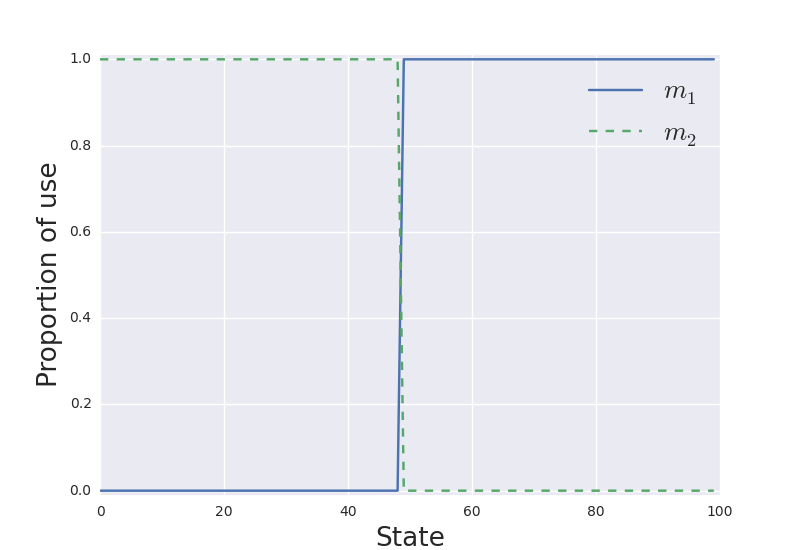
\includegraphics[scale=0.4]{../code/plots/vag-gen0.png}
    \caption{Initial non-vague population}
    \label{fig:vaga}
  \end{subfigure}
  ~
   \begin{subfigure}[b]{0.45\textwidth}
    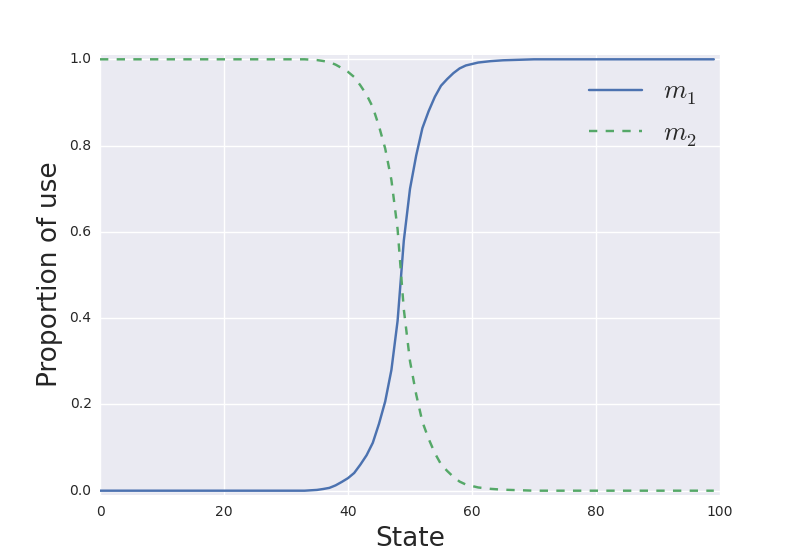
\includegraphics[scale=0.4]{../code/plots/vag-gen1.png}
    \caption{Vague population after single generation}
    \label{fig:vagb}

  \end{subfigure}
  \caption{Noisy iterated learning with posterior sampling, $\sigma = 0.4$, $k = 20$ and $100$ sampled production sequences per type.}
  \label{fig:vag}
\end{figure}
 
\paragraph{Discussion.}
In a nutshell, transmission perturbations caused by the systematic noisy perception of states reliably give rise to vagueness even if no borderline cases were initially part of a population's language. Of course, the stabilization of a linguistic system on a particular vague/clear state partition may reasonably be expected to depend not only on the effects of learning, but also on the functional (dis)advantages that such partition brings about for its users. That is, functional pressure may be necessary for borderline cases to be kept in check. Amongst others \tb{briefly mention other factors that have been argued to lead to vagueness with references}. In particular, \citet{franke+correia:toappear} have recently shown how noisy perception may lead to vagueness under functional pressure alone. Which of these factors or combination thereof plays a more central role for the emergence of vagueness is an empirical question we can not address here. Instead, we see these results as adding strength to the argument that one way in which vagueness may arise is as a byproduct of interactions between agents that may occasionally err in their perception of the environment -- be it in interaction under functional pressure or in acquisition under a pressure for learnability. 


\subsection{Deflation}

\tb{Short description of deflation and relevant work}


\paragraph{Setup.} We consider a similar setup to the one above. $S = [0,99]$, each type is associated with a threshold $\theta_i$ with $i \in [0,99]$, and the noise pattern is given by $P(s_p|s_a) \sim \text{Normal}(s_{a},\sigma)$. However, we now trace the change of a single message $m$ coupled with linguistic behavior such that $P(m|s_j,\theta_i) = 1$ iff $s_j \geq \theta_t$, otherwise no message is sent. This behavior causes asymmetry in the production data as types with high $\theta$ will reserve their message only for a  small subset of the state space and otherwise remain silent. Consequently, learning also needs to be modified to take such silent observations into account. For simplicity, we assume that learners are aware of $k$ and that $P(\theta | d) \propto (\prod_{s \in d} P(m|s,\theta)) \times \text{Binom}(\text{successes} = k-|d|, \text{trials} = k, \text{succ.prob} = \sum_{s'=0}^{\theta-1} P(s'))$. As before, the former factor corresponds to the likelihood of a type producing the witnessed data.  In addition, the latter is the probability of a type not reporting $k-|d|$ events for a total of $k$ events. $P \in \Delta(S)$ is assumed to be uniform. In words, a long sequence of data consisting of mostly silence gives stronger evidence for the type producing it having a high $\theta$, even if the few state-message pairs observed in the sequence may be equally likely to be produced by lower $\theta$. 

\paragraph{Results.} The development of a monomorphic population initially consisting only of $\theta_{80}$ is shown in Figure \ref{fig:defl}. In this setup even little noise will cause the message to gradually be applied to larger portions of the state space. As with the emergence of vagueness, the speed by which meaning deflates is regulated by $\sigma$, $k$, and to lesser degree $l$. In general, more state confusion due to higher $\sigma$, shorter sequences, or less posterior maximization, will lead to more learners inferring lower $\theta$ than present in the previous generation. 

\begin{figure}[ht]
\centering
    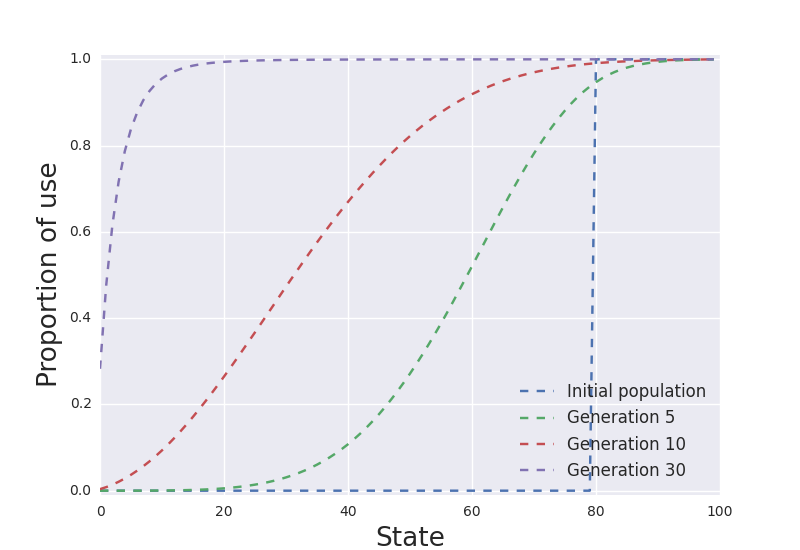
\includegraphics[scale=0.45]{../code/plots/deflation-sigma04.png}
  \caption{Noisy iterated learning with posterior sampling, $\sigma = 0.4$, $k = 30$ and $300$ sampled production sequences per type.}
  \label{fig:defl}
\end{figure}

\paragraph{Discussion.} In contrast to the previous case study, the present one considers the effects of noisy perception under an asymmetry of data generation. Teachers only gave linguistic evidence when a state held true of the message according to their type. Otherwise no overt data was given to the learner. This differs from previous studies in which each state is assumed to elicit an explicit response from the teacher, even if erroneous. This setup can instead be likened to acquisition only from positive linguistic evidence in a world in which not every state is labeled (with the idealized assumption that learners are aware of the amount of silence ``produced'' by a parent). 

The overall pattern discerned from this study is similar to that of the previous study. That is, noisy perception causes transmission perturbations that may relax once strict linguistic conventions. In contrast to the previous case study, if there are no alternative forms, e.g. {\em small} vs. {\em tall}, then asymmetry in production and noise lead will iteratively increase the state space that a message carves out, just as the overuse of a word may lead to the deflation of its meaning in natural language.


\subsection{Scalar expressions}
Scalar expressions have been at the center of many studies on conventional pragmatic inferences. Examples include quantifiers such as {\em some} and {\em most}, adjectives such as {\em cold} and {\em big}, as well as numerals such as {\em four} and {\em ten}. Their commonality lies in that their use often is taken to pragmatically convey an upper-bound that these expressions semantically lack \citep{horn:1972,gazdar:1979}. For instance, while {\em I ate some of the cookies} is truth-conditionally compatible with a state of affairs in which the speaker ate all of them, this utterance is usually reasoned to convey that the speaker ate {\em some but not all}. Otherwise, she would have used the stronger expression {\em all}. In this way, the meaning of a weak scalar expression is strengthened by speaker's and hearer's mutual reasoning about rational language use \citep{grice:1975}.

To explain the selection of a lack of upper-bounds in weak scalar expressions \citet{brochhagen+etal:2016:CogSci} proposed a model combining functional pressure and iterated learning.  Crucially, to explain this fact, this account requires the assumption of (at least a weak) prior that favors a lack of upper-bounds. Technically, this assumption is required to distinguish between a language that rules out the bound semantically and one that does so pragmatically. For brevity, let us call the former language $L_{\text{bound}}$ and the latter $L_{\text{lack}}$. To see the problem posed by $L_{\text{bound}}$, recall that learners need to infer unobservables such as linguistic behavior and a language from overt information. As a consequence, a user of $L_{\text{bound}}$ might therefore be hard or impossible to tease apart from one using $L_{\text{lack}}$ pragmatically, i.e., one that conveys the bound through pragmatic reasoning. In the following we focus on only these two languages to show under which conditions noisy perception may lead to the selection of $L_{\text{lack}}$ without a cognitive bias nor functional pressure.


\paragraph{Setup.} We use follow the setup of \citet{brochhagen+etal:2016:CogSci} but with a reduced type space by only considering $L_{\text{bound}}$ and $L_{\text{lack}}$. Both languages specify the truth-conditions for a fragment of two messages and two states. The former language partitions the state space such that $m_1$ is true of $s_1$ and $m_2$ of $s_2$. In $L_{\text{lack}}$ $m_2$ is also only true of $s_2$ but $m_1$ is true of both states, as it would be if the states were ``I ate some of the cookies'' and ``I ate all of the cookies'' and $m_1$ had the truth-conditions of {\em I ate some of the cookies}. For notational convenience we codify these truth-conditions in a Boolean matrix such that $L_{s_i,m_j} = 1$ iff $m_j$ is true of $s_i$, and otherwise $0$.

There are two types of linguistic behavior; either literal or pragmatic. The production behavior of literal types is given by $P_{\text{literal}}(m|s;L) \propto \exp(\lambda L_{sm})$. Pragmatic behavior corresponds to $P_{\text{pragmatic}}(m|s;L) \propto \exp(P_{\text{litertal}}(s|m;L))$, where $\lambda$ is a rationality parameter and $P_{\text{litertal}}(s|m;L) \propto P(s) L_{sm}$. That is, pragmatic speakers reason about their addressees to refine their linguistic choices. This allows pragmatic users of $L_{\text{lack}}$ to convey an upper-bound with $m_1$ following the reasoning spelled-out above: If they wanted to convey the stronger state $s_2$, they would have used stronger and unambiguous $m_2$ instead (c.f. \citealt{frank+goodman:2012,franke+jaeger:2014}). Finally, the rationality parameter $\lambda$ controls linguistic choice. Intuitively, higher values increase the speaker's propensity to produce utterances that maximize communicative success, i.e., to use utterances that have the highest chance of being understood. For our purposes it suffices to fix $\lambda$ to be reasonably high so as to render speaker behavior (mostly) deterministic. Combining these two types of behavior with $L_{\text{bound}}$ and $L_{\text{lack}}$ gives a total of four different types.

Lastly, and differently from Brochhagen et al.'s noise-free model, noise is introduced by two parameters $\epsilon$ and $\delta$. The former corresponds to the probability of perceiving an actual state $s_1$ as $s_2$, $P(s_1 | s_2) = \epsilon$, and conversely $P(s_2 | s_1) = \delta$.

\paragraph{Results.} To quantify the effects of the dynamics we ran $50$ independent simulations per parameter configuration. Each population was initialized with an arbitrary distribution over types. The mean proportion of pragmatic users of $L_{\text{lack}}$ under different noise signatures is shown in Figure \ref{fig:quant}. These results show that when $\delta$ is small and $\epsilon$ is high, iterated noisy transmission can lead to populations consisting of mostly, if not exclusively, types that lexicalize no upper-bounds in for their weak scalar expressions provided language users are pragmatic.  Similar results are obtained for increments of $k$ or $l$. 

\begin{figure}[ht]
\centering
    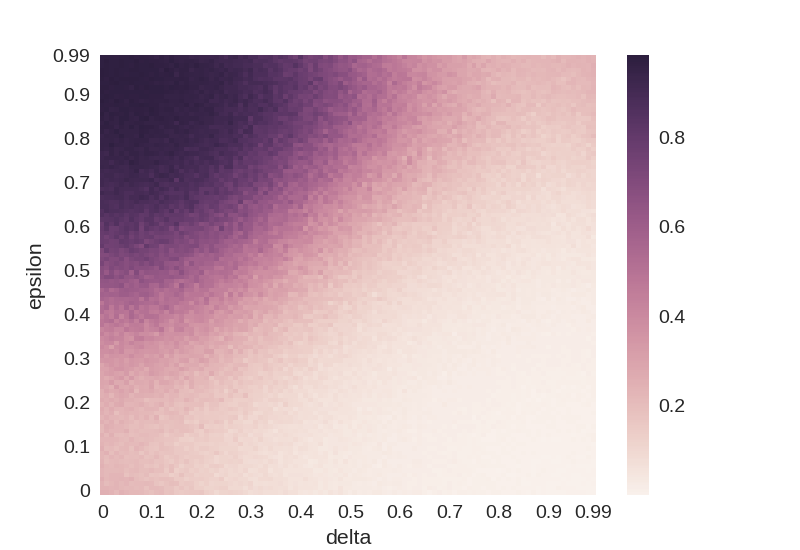
\includegraphics[scale=0.5]{../code/plots/quantifiers-posterior-sampling-k5.png}
  \caption{Mean proportion of pragmatic $L_{\text{lack}}$ users after $20$ generations with posterior sampling, $k = 5, \lambda = 20$ and $10$ sampled production sequences per parent type. \tb{Axes should be $\delta$ and $\epsilon$.}}
  \label{fig:quant}
\end{figure}


\paragraph{Discussion.} The main purpose of this case study is to show that noisy perception can mimic the effect of cognitive biases. In the case of Brochhagen et al. the assumed bias was one for simplicity. Accordingly, learners had an a priori preference for not codifying an upper-bound lexically over codifying it. As noted above, this influenced the propensity of learners to infer pragmatic $L_{\text{lack}}$ over $L_{\text{bound}}$ even if the evidence provided by the data could not tease them apart. Here, we assumed no such bias but nevertheless arrived at an evolutionary outcome that is comparable to the one predicted if it were present. However, this outcome strongly depends on the types involved. Whether a type thrives under a particular noise pattern depends on the proportion of types confused with it during transmission. The addition or extraction of a single type may therefore lead to different results. \tb{Maybe mention explicitly that it doesn't work with the full space. Add some discussion on the relation between noise and quantifiers/scalar expressions}


\section{Discussion}
\tb{TO DO} 

\section{Conclusion}
\tb{TO DO}

\section{Acknowledgments}
\tb{TO DO}


\bibliographystyle{apacite}

\setlength{\bibleftmargin}{.125in}
\setlength{\bibindent}{-\bibleftmargin}

\bibliography{noise-bib}


\end{document}
